\documentclass[crop,tikz,convert={outext=.svg,command=\unexpanded{pdf2svg \infile\space\outfile}},multi=false]{standalone}[2012/04/13]
\usetikzlibrary{arrows}
\begin{document}
            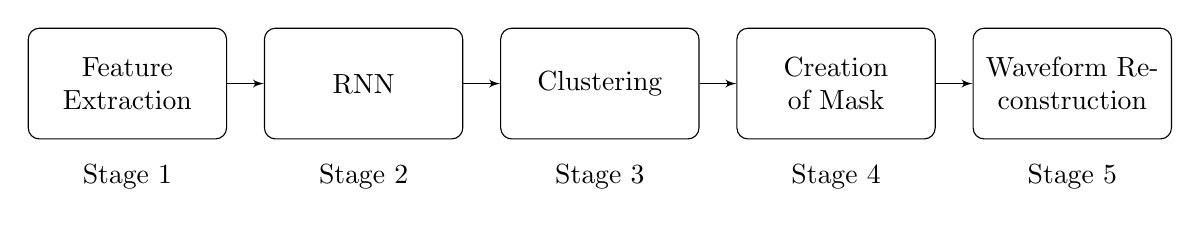
\begin{tikzpicture}[node distance = 3cm, label distance=2mm, auto]
                \tikzstyle{block} = [rectangle, draw, text width=6.5em, text centered, rounded corners, minimum height=4em]
                \tikzstyle{line} = [draw, -latex']
                % Place nodes
                \node [block, label=below:Stage 1] (feature) {Feature Extraction};
                \node [block, label=below:Stage 2, right of=feature] (rnn) {RNN};
                \node [block, label=below:Stage 3, right of=rnn] (clustering) {Clustering};
                \node [block, label=below:{Stage 4}, right of=clustering] (masking) {Creation of Mask};
                \node [block, label=below:Stage 5, right of=masking] (reconstruction) {Waveform Reconstruction};
                % Draw edges
                \path [line] (feature) -- (rnn);
                \path [line] (rnn) -- (clustering);
                \path [line] (clustering) -- (masking);
                \path [line] (masking) -- (reconstruction);
            \end{tikzpicture}
\end{document}
